% ---------------------------------------------------------------------------
% fig_group_size.tex
% Trainability and held-out performance vs group size G.
% The relationship is NON-MONOTONE: the headline GSM8K sweep peaks at the
% intermediate G=8 and collapses at G=16, while the confirmation sweep's train
% reward rises and its mean ZVF falls monotonically in G.
% DATA:
%   paper/expected_results.json                -> panel (a): headline G-sweep
%   experiments/results/group_size_effect.tsv  -> panels (b), (c), (d)
% INTEGRITY (do not remove):
%   (a) is a SINGLE-SEED, 30-step sweep -> no error bars are possible and it
%       cannot establish an optimum. Labelled as such inside the panel.
%   (b) is the measured n=3 confirmation sweep; its held-out apex is NOT
%       statistically separable from its neighbours (overlapping SEs), so the
%       supported claim is only that the optimum is interior.
%   Every plotted value is a cell of the cited file; nothing is invented.
% ---------------------------------------------------------------------------
\documentclass[border=6pt]{standalone}
\usepackage{tikz}
\usepackage{pgfplots}
\pgfplotsset{compat=1.18}
\usetikzlibrary{arrows.meta,positioning,shapes.geometric,fit,backgrounds,calc,decorations.pathreplacing,patterns}
\usetikzlibrary{pgfplots.groupplots}
\tikzset{
  blk/.style={rectangle, rounded corners=2pt, draw=black!70, thick, fill=blue!6,
              minimum height=8mm, minimum width=20mm, align=center, font=\small},
  io/.style={rectangle, rounded corners=6pt, draw=black!70, thick, fill=green!8,
             minimum height=8mm, align=center, font=\small},
  proc/.style={rectangle, draw=black!70, thick, fill=orange!10, minimum height=8mm,
               align=center, font=\small},
  dec/.style={diamond, aspect=2, draw=black!70, thick, fill=yellow!15, align=center, font=\footnotesize},
  warnbox/.style={rectangle, rounded corners=2pt, draw=red!60!black, thick, fill=red!7,
                  minimum height=8mm, align=center, font=\small},
  oklbox/.style={rectangle, rounded corners=2pt, draw=green!45!black, thick, fill=green!8,
                 minimum height=8mm, align=center, font=\small},
  ar/.style={-{Latex[length=2mm]}, thick},
  arl/.style={-{Latex[length=2mm]}, thick, dashed, draw=black!55},
  lbl/.style={font=\footnotesize\itshape, text=black!60},
}
\definecolor{good}{RGB}{34,139,34}
\definecolor{bad}{RGB}{178,34,34}
\definecolor{warn}{RGB}{218,165,32}
\definecolor{pesblue}{RGB}{0,45,98}
\definecolor{complete}{RGB}{30,125,79}
\definecolor{partial}{RGB}{176,106,0}
\definecolor{blocked}{RGB}{166,43,43}
\begin{document}
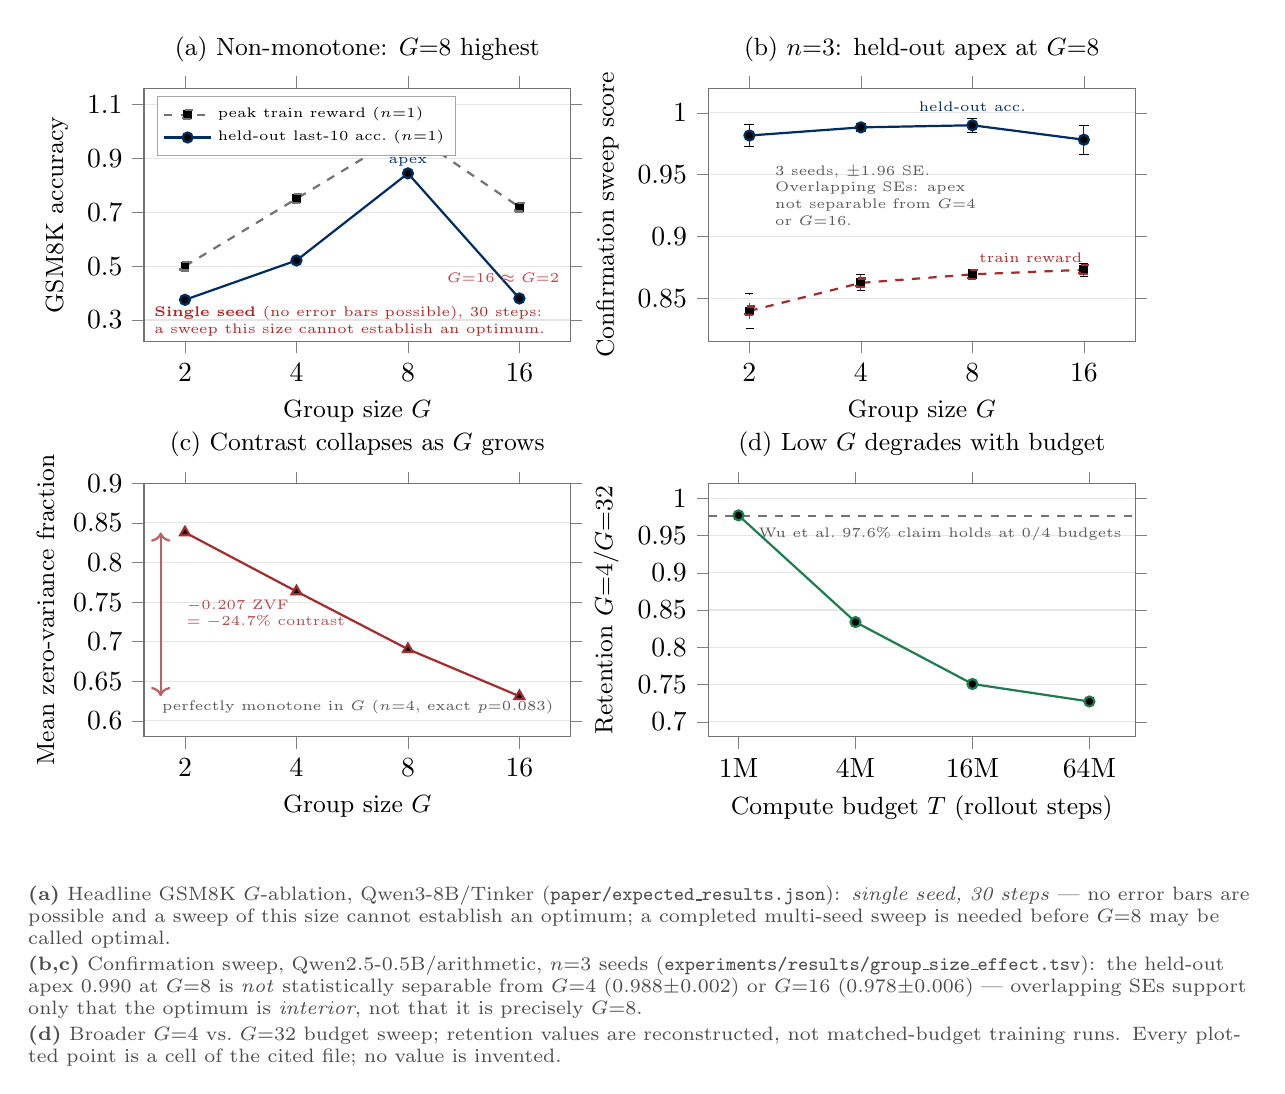
\begin{tikzpicture}
\begin{groupplot}[
  group style={group size=2 by 2, horizontal sep=1.75cm, vertical sep=1.8cm},
  width=7.0cm, height=4.8cm,
  xmode=log,
  xtick={2,4,8,16}, xticklabels={2,4,8,16},
  xmin=1.55, xmax=22,
  ymajorgrids, grid style={black!10},
  axis line style={draw=black!55},
  tick align=outside,
  label style={font=\small},
  title style={font=\small},
  legend style={font=\tiny, draw=black!35, fill=white, cells={anchor=west},
                row sep=-1pt, inner sep=2pt},
  s1/.style={thick, mark=*, mark size=1.8pt},
  s2/.style={thick, dashed, mark=square*, mark size=1.6pt},
  s3/.style={thick, mark=triangle*, mark size=2.0pt},
]
% ============ (a) headline GSM8K G-sweep: NON-MONOTONE, single seed =========
\nextgroupplot[
  ymin=0.22, ymax=1.16,
  ytick={0.3,0.5,0.7,0.9,1.1},
  ylabel={GSM8K accuracy},
  xlabel={Group size $G$},
  title={(a) Non-monotone: $G{=}8$ highest},
  legend pos=north west,
]
\addplot[s2, draw=black!55] coordinates {
  (2,0.500) (4,0.750) (8,1.000) (16,0.719)
};
\addlegendentry{peak train reward ($n{=}1$)}
\addplot[s1, draw=pesblue] coordinates {
  (2,0.375) (4,0.521) (8,0.844) (16,0.380)
};
\addlegendentry{held-out last-10 acc.\ ($n{=}1$)}
\node[anchor=south, font=\tiny, text=pesblue, inner sep=1pt]
     at (axis cs:8,0.860) {apex};
\node[anchor=south east, font=\tiny, text=bad!85]
     at (axis cs:21.8,0.400) {$G{=}16 \approx G{=}2$};
\node[anchor=south west, align=left, font=\tiny, text=bad, inner sep=1pt]
     at (axis cs:1.62,0.228) {\textbf{Single seed} (no error bars possible), 30 steps:\\
      a sweep this size cannot establish an optimum.};
% ==== (b) n=3 confirmation: held-out non-monotone, train reward monotone =====
\nextgroupplot[
  ymin=0.815, ymax=1.020,
  ytick={0.85,0.90,0.95,1.00},
  yticklabel style={/pgf/number format/fixed,
                    /pgf/number format/precision=2,
                    /pgf/number format/assume math mode=true},
  ylabel={Confirmation sweep score},
  xlabel={Group size $G$},
  title={(b) $n{=}3$: held-out apex at $G{=}8$},
  error bars/y dir=both, error bars/y explicit,
]
\addplot[s1, draw=pesblue]
  coordinates {
  (2,0.9817) +- (0,0.0086)
  (4,0.9883) +- (0,0.0033)
  (8,0.9900) +- (0,0.0057)
  (16,0.9783) +- (0,0.0118)
};
\addplot[s2, draw=blocked]
  coordinates {
  (2,0.8398) +- (0,0.0141)
  (4,0.8625) +- (0,0.0065)
  (8,0.8694) +- (0,0.0037)
  (16,0.8731) +- (0,0.0053)
};
\node[anchor=south, font=\tiny, text=pesblue, inner sep=1pt]
     at (axis cs:8,0.9985) {held-out acc.};
\node[anchor=south, font=\tiny, text=blocked, inner sep=1pt]
     at (axis cs:11.5,0.8765) {train reward};
\node[anchor=north west, align=left, font=\tiny, text=black!65, inner sep=1pt]
     at (axis cs:2.30,0.9600) {3 seeds, $\pm1.96$ SE.\\ Overlapping SEs: apex\\ not separable from $G{=}4$\\ or $G{=}16$.};
% ============ (c) mean ZVF falls monotonically ==============================
\nextgroupplot[
  ymin=0.58, ymax=0.90,
  ytick={0.6,0.65,0.7,0.75,0.8,0.85,0.9},
  ylabel={Mean zero-variance fraction},
  xlabel={Group size $G$},
  title={(c) Contrast collapses as $G$ grows},
]
\addplot[s3, draw=blocked] coordinates {
  (2,0.838) (4,0.7635) (8,0.6906) (16,0.6312)
};
\draw[<->, thick, draw=blocked!75] (axis cs:1.72,0.6312) -- (axis cs:1.72,0.838);
\node[anchor=west, font=\tiny, text=blocked!85, align=left]
     at (axis cs:1.90,0.735) {$-0.207$ ZVF\\$=-24.7\%$ contrast};
\node[anchor=south east, font=\tiny, text=black!65, align=right]
     at (axis cs:21,0.596) {perfectly monotone in $G$ ($n{=}4$, exact $p{=}0.083$)};
% ============ (d) small G does not hold up as compute grows =================
\nextgroupplot[
  xtick={1000000,4000000,16000000,64000000},
  xticklabels={1M,4M,16M,64M},
  xmin=700000, xmax=110000000,
  ymin=0.68, ymax=1.02,
  ytick={0.7,0.75,0.8,0.85,0.9,0.95,1.0},
  ylabel={Retention $G{=}4/G{=}32$},
  xlabel={Compute budget $T$ (rollout steps)},
  title={(d) Low $G$ degrades with budget},
]
\addplot[s1, draw=complete] coordinates {
  (1000000,0.9770) (4000000,0.8339) (16000000,0.7508) (64000000,0.7273)
};
\draw[dashed, thick, draw=black!55] (axis cs:700000,0.976) -- (axis cs:110000000,0.976);
\node[anchor=east, font=\tiny, text=black!65]
     at (axis cs:105000000,0.952) {Wu et al.\ 97.6\% claim holds at $0/4$ budgets};
\end{groupplot}
\node[anchor=north west, text width=15.6cm, font=\scriptsize, text=black!70,
      align=left, inner sep=0pt]
     at ([yshift=-7mm]current bounding box.south west) {%
  \textbf{(a)} Headline GSM8K $G$-ablation, Qwen3-8B/Tinker
  (\texttt{paper/expected\_results.json}): \emph{single seed, 30 steps} --- no error bars are
  possible and a sweep of this size cannot establish an optimum; a completed multi-seed sweep is
  needed before $G{=}8$ may be called optimal.
  \\[0.4ex]
  \textbf{(b,c)} Confirmation sweep, Qwen2.5-0.5B/arithmetic, $n{=}3$ seeds
  (\texttt{experiments/results/group\_size\_effect.tsv}): the held-out apex $0.990$ at $G{=}8$ is
  \emph{not} statistically separable from $G{=}4$ ($0.988{\pm}0.002$) or $G{=}16$ ($0.978{\pm}0.006$)
  --- overlapping SEs support only that the optimum is \emph{interior}, not that it is precisely $G{=}8$.
  \\[0.4ex]
  \textbf{(d)} Broader $G{=}4$ vs.\ $G{=}32$ budget sweep; retention values are reconstructed, not
  matched-budget training runs. Every plotted point is a cell of the cited file; no value is invented.};
\end{tikzpicture}
\end{document}
